% Whittle Laboratory Beamer Template
% Based on the University of Cambridge Powerpoint Template
% J. Brind
% May 2016

%%%%%%%%%%%%%%%%%%%
% TEMPLATE SET UP %
%%%%%%%%%%%%%%%%%%%

% Use Beamer and the Cambridge theme
\documentclass{beamer}
\usetheme{cambridge}

% New slide numbers for the appendix
\usepackage{appendixnumberbeamer}

\usepackage{amssymb}

% helvetica font
\usepackage{helvet}

% equations in black
\usefonttheme[onlymath]{serif}

% this package ensures words with umlauts etc. in are properly hyphenated!
\usepackage[T1]{fontenc}

% footer reference box definition
\usepackage[absolute,overlay]{textpos}
\newcommand{\footreftwo}[1]{%
 \begin{textblock*}{7.8cm}(2.75cm,8.54cm)%
    \vspace{0.05em}\flushleft \colorlet{saved}{.}\color{white} \tiny #1 \color{saved}
  \end{textblock*}
}

\newcommand{\footrefthree}[1]{%
 \begin{textblock*}{7.8cm}(2.75cm,8.43cm)%
    \vspace{0.05em}\flushleft \colorlet{saved}{.}\color{white} \tiny #1 \color{saved}
  \end{textblock*}
}


% redefinitions for vertical centering of list items
% still need extra vfills sometimes
%\let\olditem\item
%\renewcommand{\item}{\setlength{\itemsep}{\fill}\olditem}

%%%%%%%%%%%%%%%%%%%%%
% OPTIONAL PACKAGES %
%%%%%%%%%%%%%%%%%%%%%

% Personal packages
\usepackage{siunitx}
\sisetup{range-units=single}

% Personal TeX macros
\newcommand{\etal}{\emph{et al.\@} }
\newcommand{\BR}{\mathit{BR}}
\newcommand{\IR}{\mathit{IR}}
\newcommand{\DR}{\mathit{DR}}
\newcommand{\Rey}{\mathit{Re}}
\newcommand*\df{\mathop{}\!\mathrm{d}}
\newcommand*\Df{\mathop{}\!\mathrm{D}}

% for absolute positioning
\def\Put(#1,#2)#3{\leavevmode\makebox(0,0){\put(#1,#2){#3}}}

%%%%%%%%%%%%%%%%%%%%%%%
% Author, Title, etc. %
%%%%%%%%%%%%%%%%%%%%%%%

\title{Example presentation}

%\subtitle{beansg}

\author{\texorpdfstring{\textbf{James Brind}}{James Brind} \\ 
Whittle Laboratory \\
University of Cambridge \\
Cambridge, CB3 0DY, UK \\
Email: jb753@cam.ac.uk}

\date{\today}

%%%%%%%%%%%%%%%%%%%%%%%%%%% The main document %%%s%%%%%%%%%%%%%%%%%%%%%%%%%%%


\begin{document}

%
% TITLE SLIDE
%
\begin{frame}
  \titlepage
\end{frame}

%
% MOTIVATION
%
\begin{frame}{Example Figure}
  \centering
  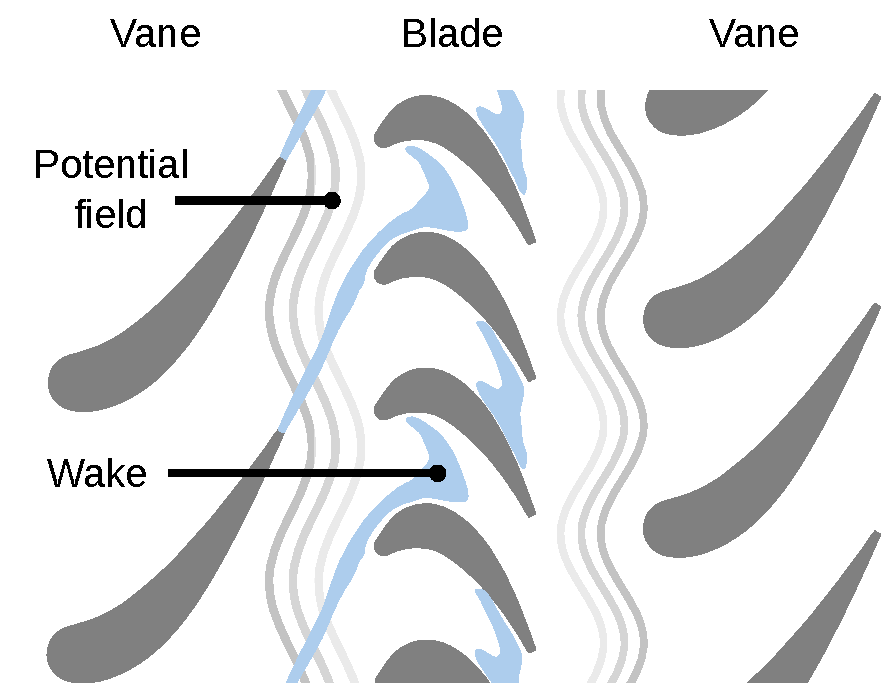
\includegraphics[width=0.9\linewidth,trim={0 1.5cm 0 0},clip]{figures/blade_row_interactions.pdf}
\end{frame}

\part{Example Part}
\frame{\partpage}

\begin{frame}{Itemize}
  \begin{itemize}
    \item item
    \item item
   \alert{\item alert}
  \end{itemize}
\end{frame}

\begin{frame}{Block environments}
  \begin{block}{Block}
    This is a block.\\
    A block with two lines.
  \end{block}
  \begin{exampleblock}{Example}
    This is an example.
  \end{exampleblock}

\end{frame}

\begin{frame}{Theorems}

  \begin{theorem}[Author]
    This is a theorem.\\
    \[ a^2 = b^2 + c^2\]
  \end{theorem}
  \begin{definition}
    This is a theorem.\\
    \[ a^2 = b^2 + c^2\]
  \end{definition}

\footrefthree{A three line reference. A three line reference. A three line reference. A three line reference. A three line reference. A three line reference. A three line reference. A three line reference. A three line reference. }


\end{frame}

\begin{frame}{Proof}

  \begin{proof}[My proof]
    This is a proof.\\
  \end{proof}

\footreftwo{A two line reference. A two line reference. A two line reference. A two line reference. A two line reference. A two line reference. A two line reference. }

\end{frame}

\begin{frame}{Columns}
  \dblcol{Bottom\vfill Top}{Test}
\end{frame}


\end{document}


